\documentclass[9pt]{article}
\usepackage[left=.5in, right=.5in, top=1in]{geometry}

\usepackage{graphicx}					
\usepackage{amssymb}
\usepackage{float}
\usepackage{url}
\usepackage{graphicx}					
\usepackage{import}
\usepackage{dcolumn}
\usepackage{amssymb}
\usepackage{adjustbox}
\graphicspath{ {Results/} }

\title{Results}
\author{.}

% ------------------------------------------------------------------------------------
\begin{document}

\maketitle
%\tableofcontents

% ------------------------------------------------------------------------------------
\newpage
\section{Main Results}

%%
\begin{figure}[H]
\centering
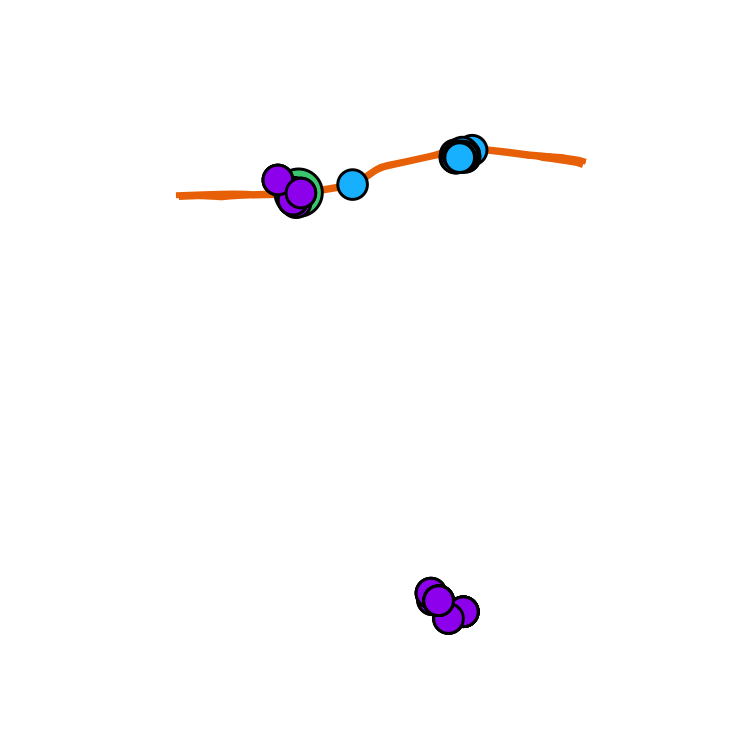
\includegraphics[width=0.3\textwidth]{figures/figure_1a.png}
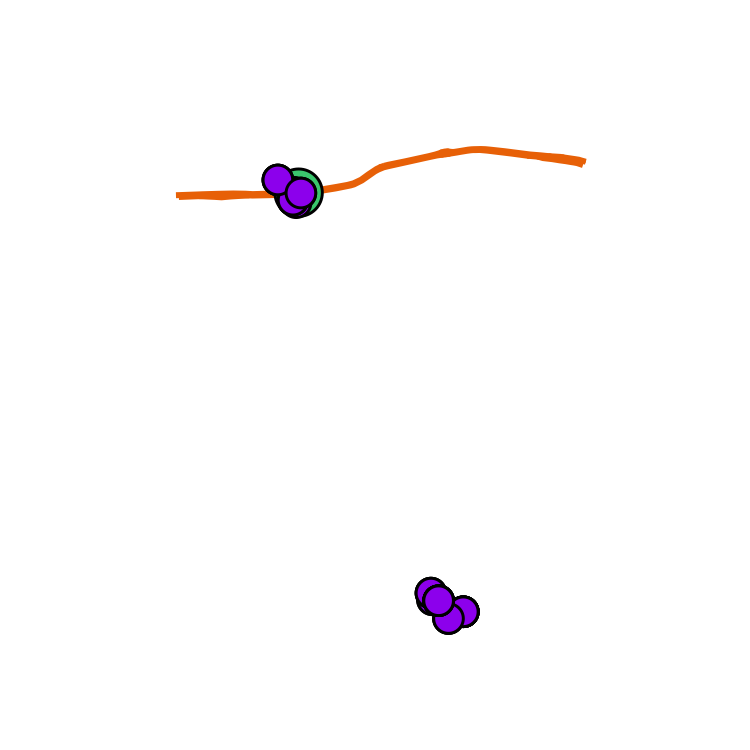
\includegraphics[width=0.3\textwidth]{figures/figure_1b.png}
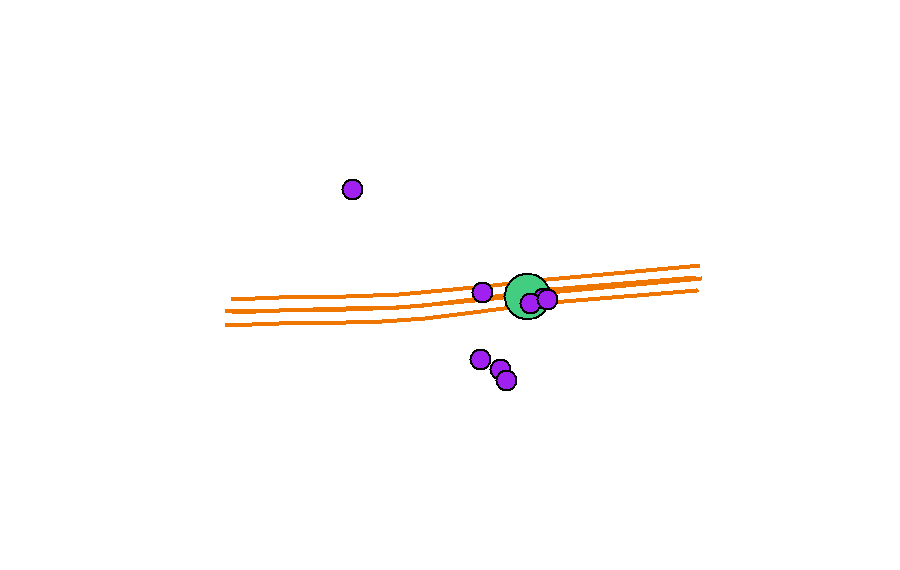
\includegraphics[width=0.3\textwidth]{figures/figure_1c.png}
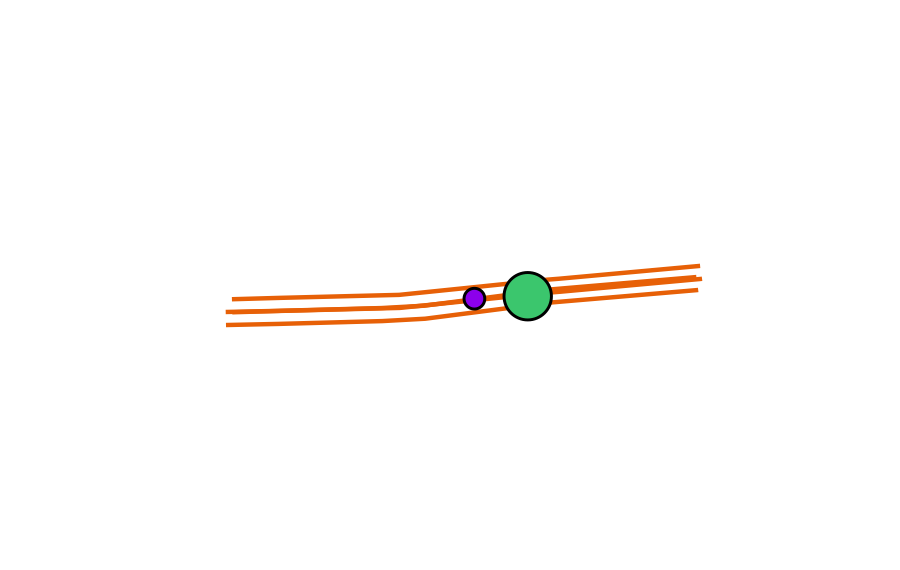
\includegraphics[width=0.3\textwidth]{figures/figure_1d.png}
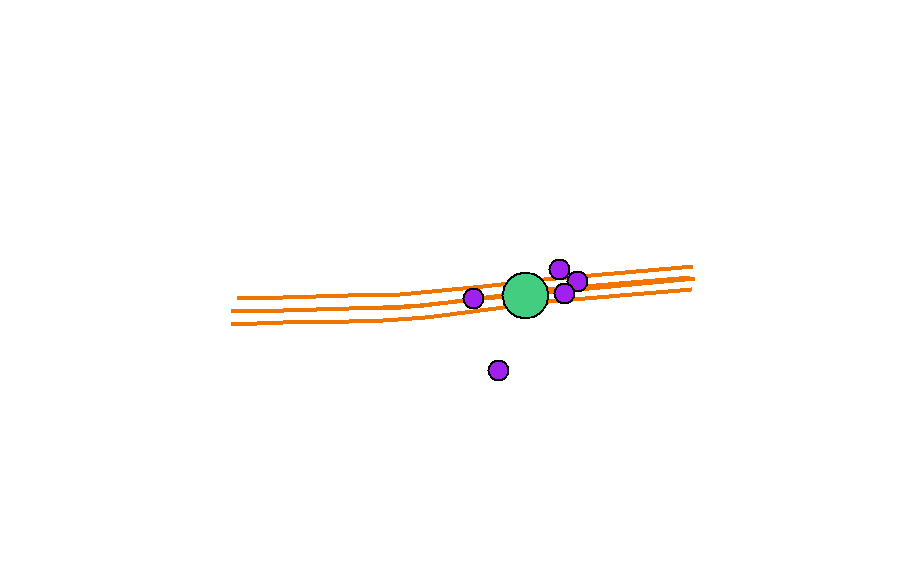
\includegraphics[width=0.3\textwidth]{figures/figure_1e.png}
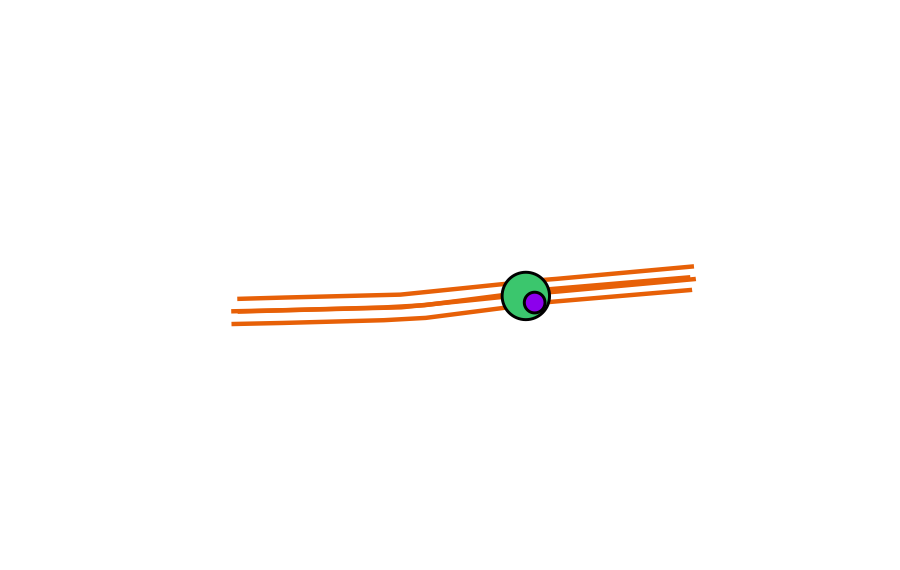
\includegraphics[width=0.3\textwidth]{figures/figure_1f.png}
\caption{In Paper: Figure 1}
\end{figure}

\begin{table}[H]
\caption{In Paper: Table 1}
\centering
\begin{tabular}{l cc | cc} \hline  & \multicolumn{2}{c|}{Any Location} & \multicolumn{2}{c}{Crash Location } \\  & \multicolumn{2}{c|}{Captured by} & \multicolumn{2}{c}{Determined by} \\  & \multicolumn{2}{c|}{Algorithm Close to} & \multicolumn{2}{c}{Algorithm Close to} \\  & \multicolumn{2}{c|}{True Crash Location} & \multicolumn{2}{c}{True Crash Location} \\  \hline  & Recall & Precision & Recall & Precision \\ \hline LNEx & 0.674  & 0.686  & 0.129  & 0.132  \\ Alg., Raw Gaz & 0.695  & 0.757  & 0.579  & 0.756  \\ Alg., Aug Gaz & 0.798  & 0.857  & 0.651  & 0.811  \\ Alg., Aug Gaz [Cluster] &  & & 0.656  & 0.774  \\ \hline \multicolumn{5}{p{11cm}}{`N Crashes' refers to the number of correctly 
    identified crashes. `Raw Gaz' refers to the raw gazetteer (ie, dictionary of 
    landmarks with original names) and `Aug Gaz' refers to the augmented gazetteer. 
    We use our raw gazetteer as an input into LNEX, which implements its own augmentation
    process. For LNEx, the crash location is determined by taking the centroid of all 
    locations captured by the algorithm. Locations are considered close if they are 
    within 500 meters of each other.} \end{tabular} 
\end{table}

\begin{figure}[H]
\centering
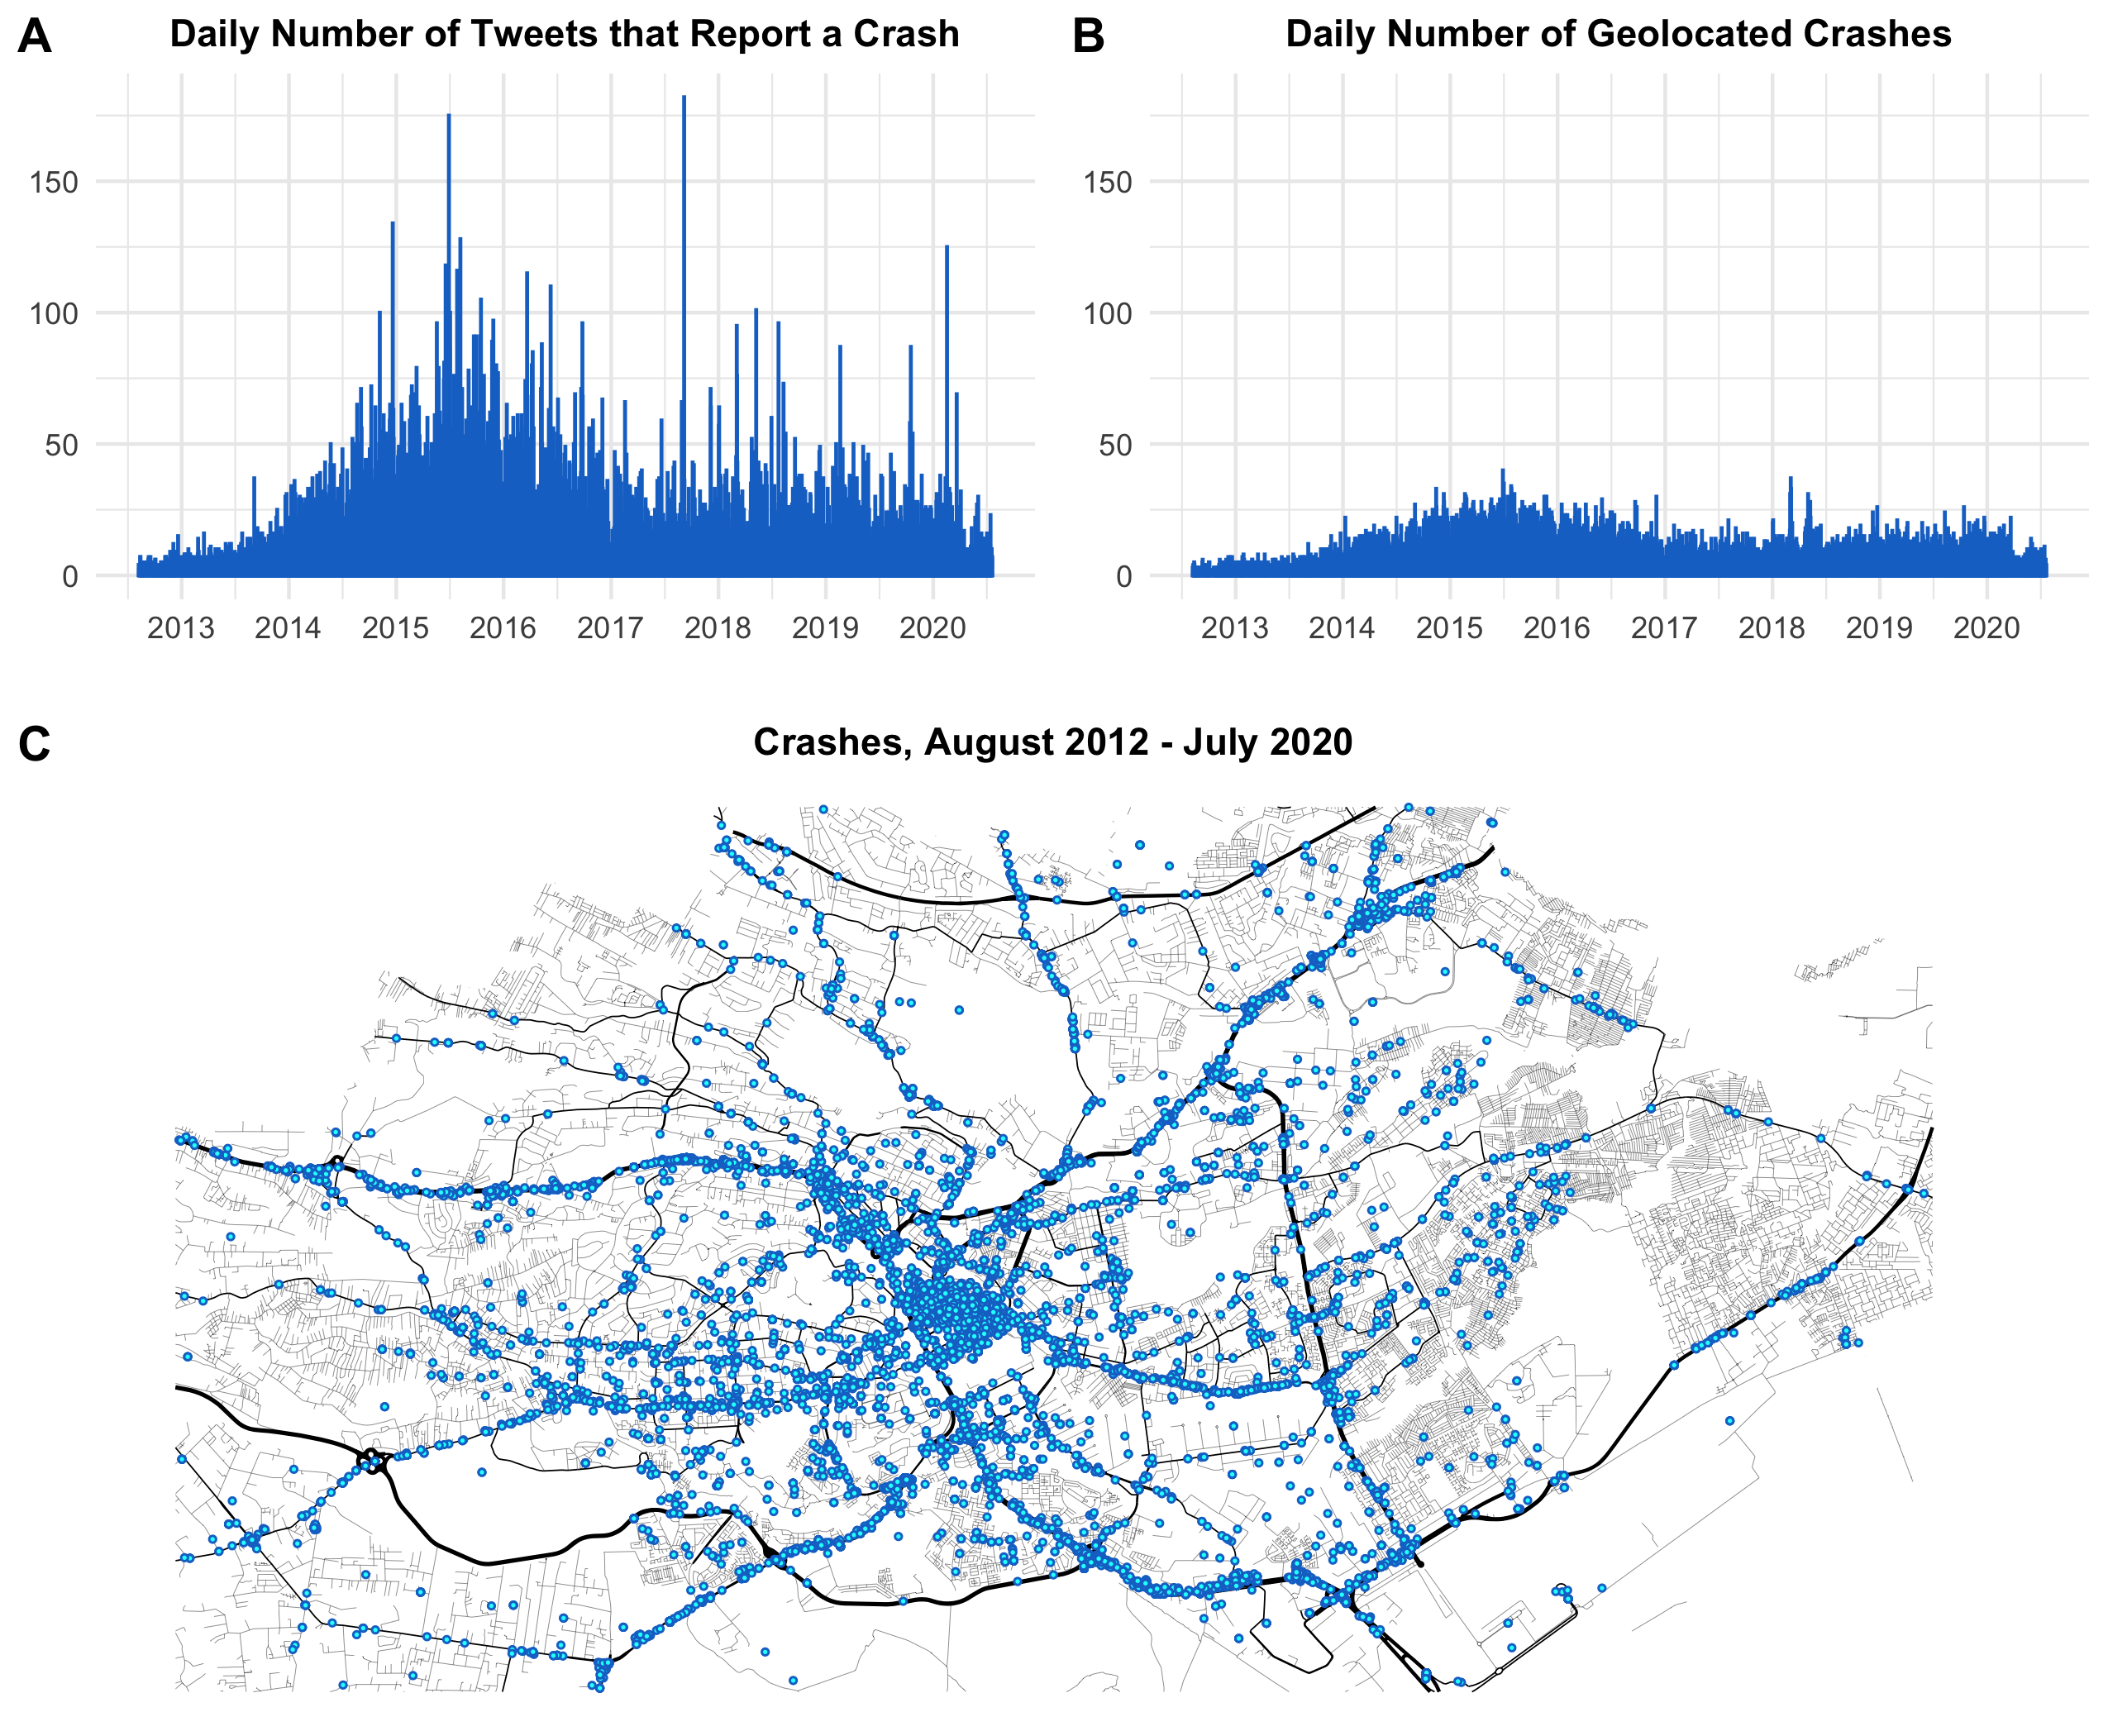
\includegraphics[width=0.75\textwidth]{figures/figure_2.png}
\caption{In Paper: Figure 2}
\end{figure}

\begin{figure}[H]
\centering
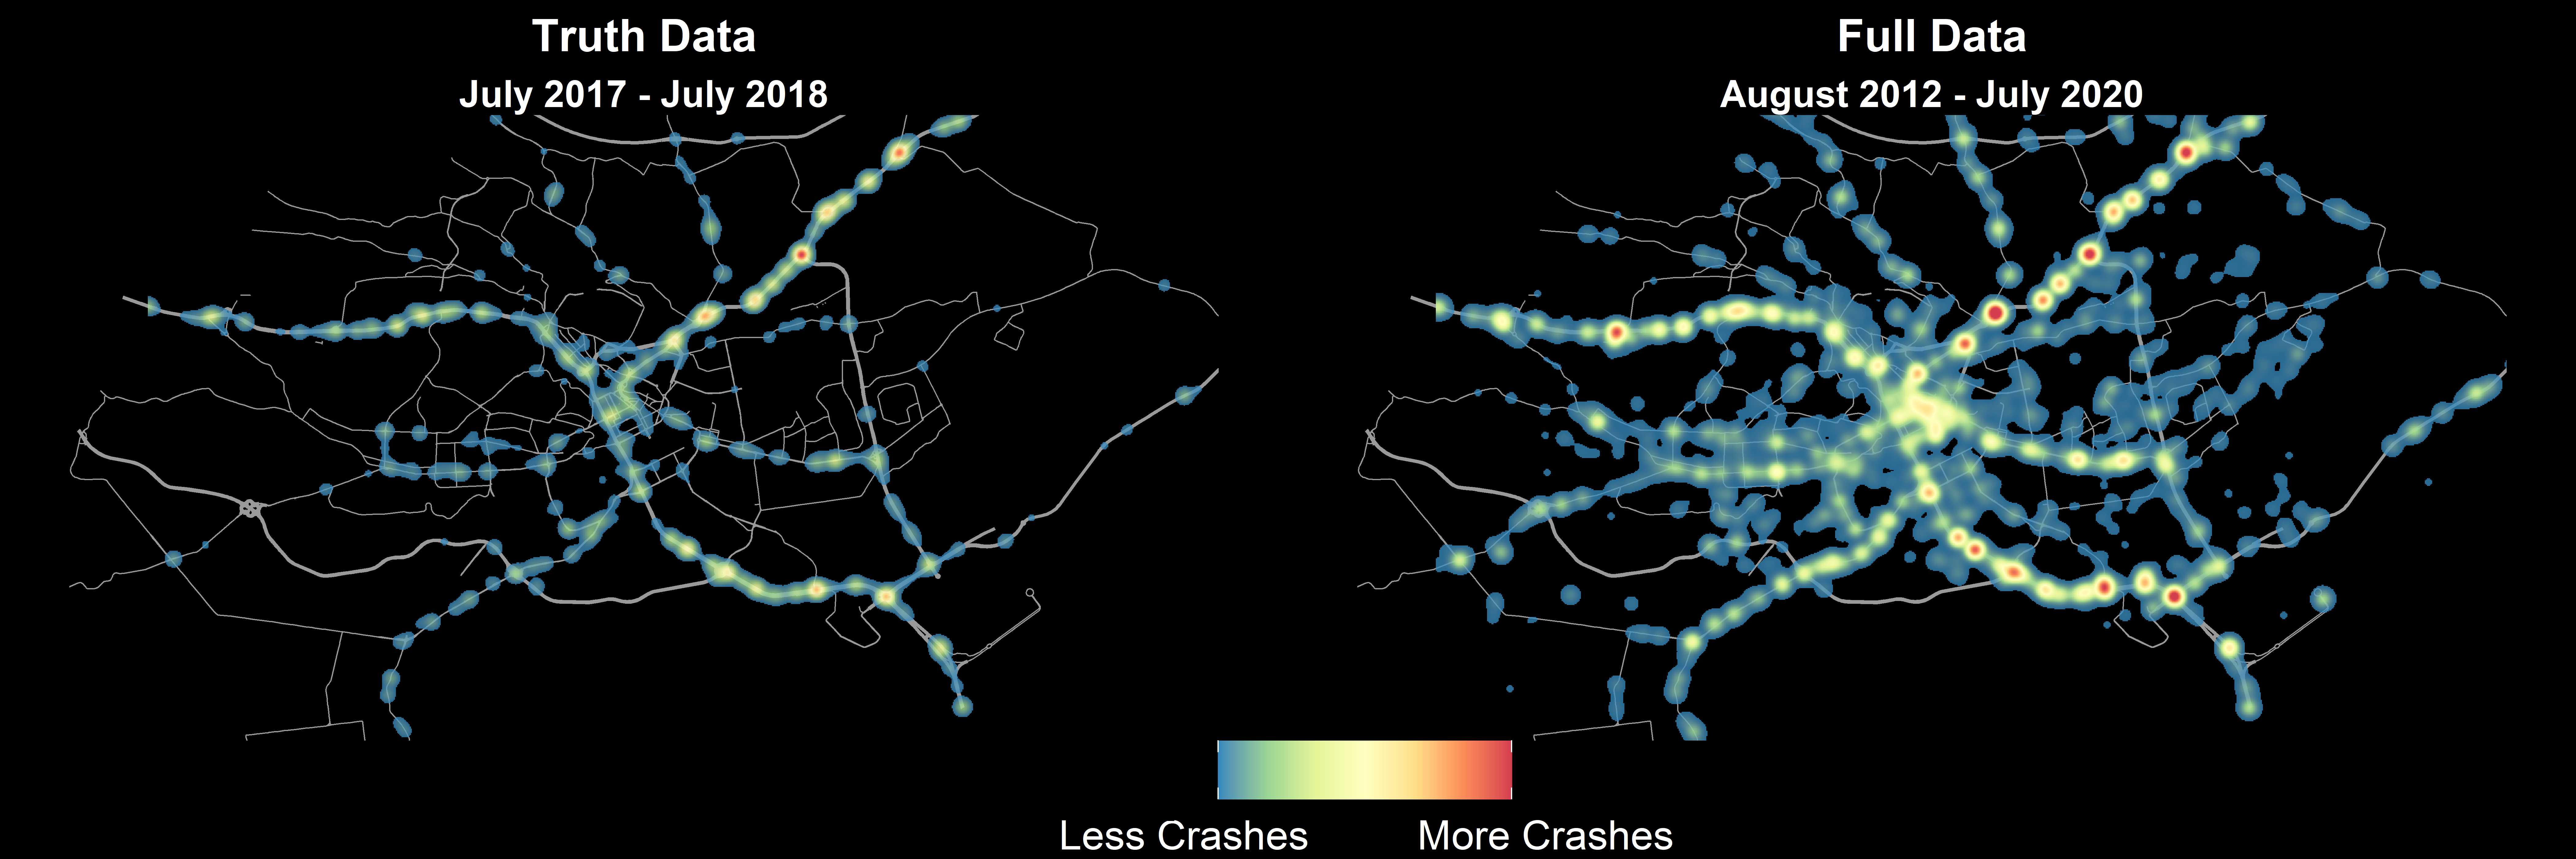
\includegraphics[width=0.75\textwidth]{figures/figure_3.png}
\caption{In Paper: Figure 3}
\end{figure}

% ------------------------------------------------------------------------------------
\newpage
\section{Supplementary Information}

\begin{figure}[H]
\centering
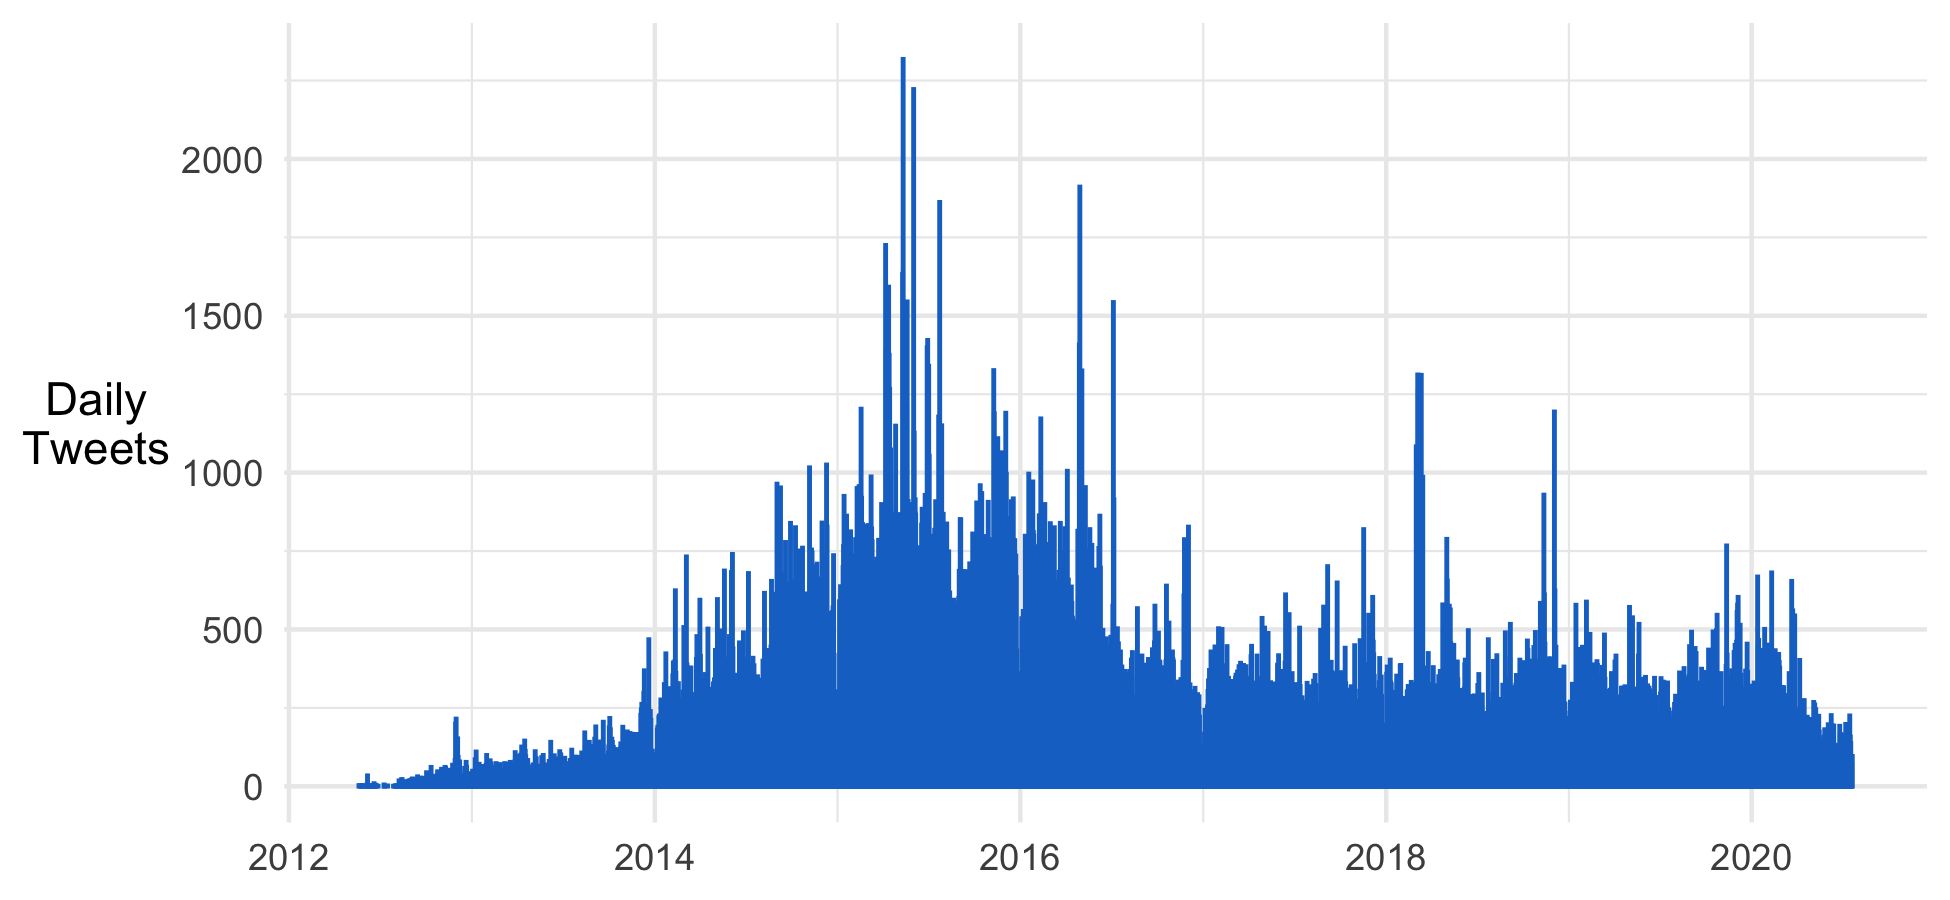
\includegraphics[width=0.75\textwidth]{figures/figure_s1.png}
\caption{In Paper: Figure s1}
\end{figure}

\begin{table}[H]
\caption{In Paper: Table s4}
\centering
 \begin{tabular}{cccc | c}  \hline Precision & Recall & F1 & Accuracy & N-Grams \\  \hline \multicolumn{4}{c|}{Naive Bayes} &  \\ 0.938 & 0.947 & 0.942 & 0.919 & 1  \\  0.945 & 0.949 & 0.947 & 0.926 & 2  \\  0.945 & 0.949 & 0.947 & 0.926 & 3  \\  \hline \multicolumn{4}{c|}{SVM} &  \\ 0.935 & 0.963 & 0.948 & 0.927 & 1  \\  0.94 & 0.966 & 0.953 & 0.934 & 2  \\  0.939 & 0.967 & 0.953 & 0.934 & 3  \\  \hline \end{tabular}
\end{table}

\begin{figure}[H]
\centering
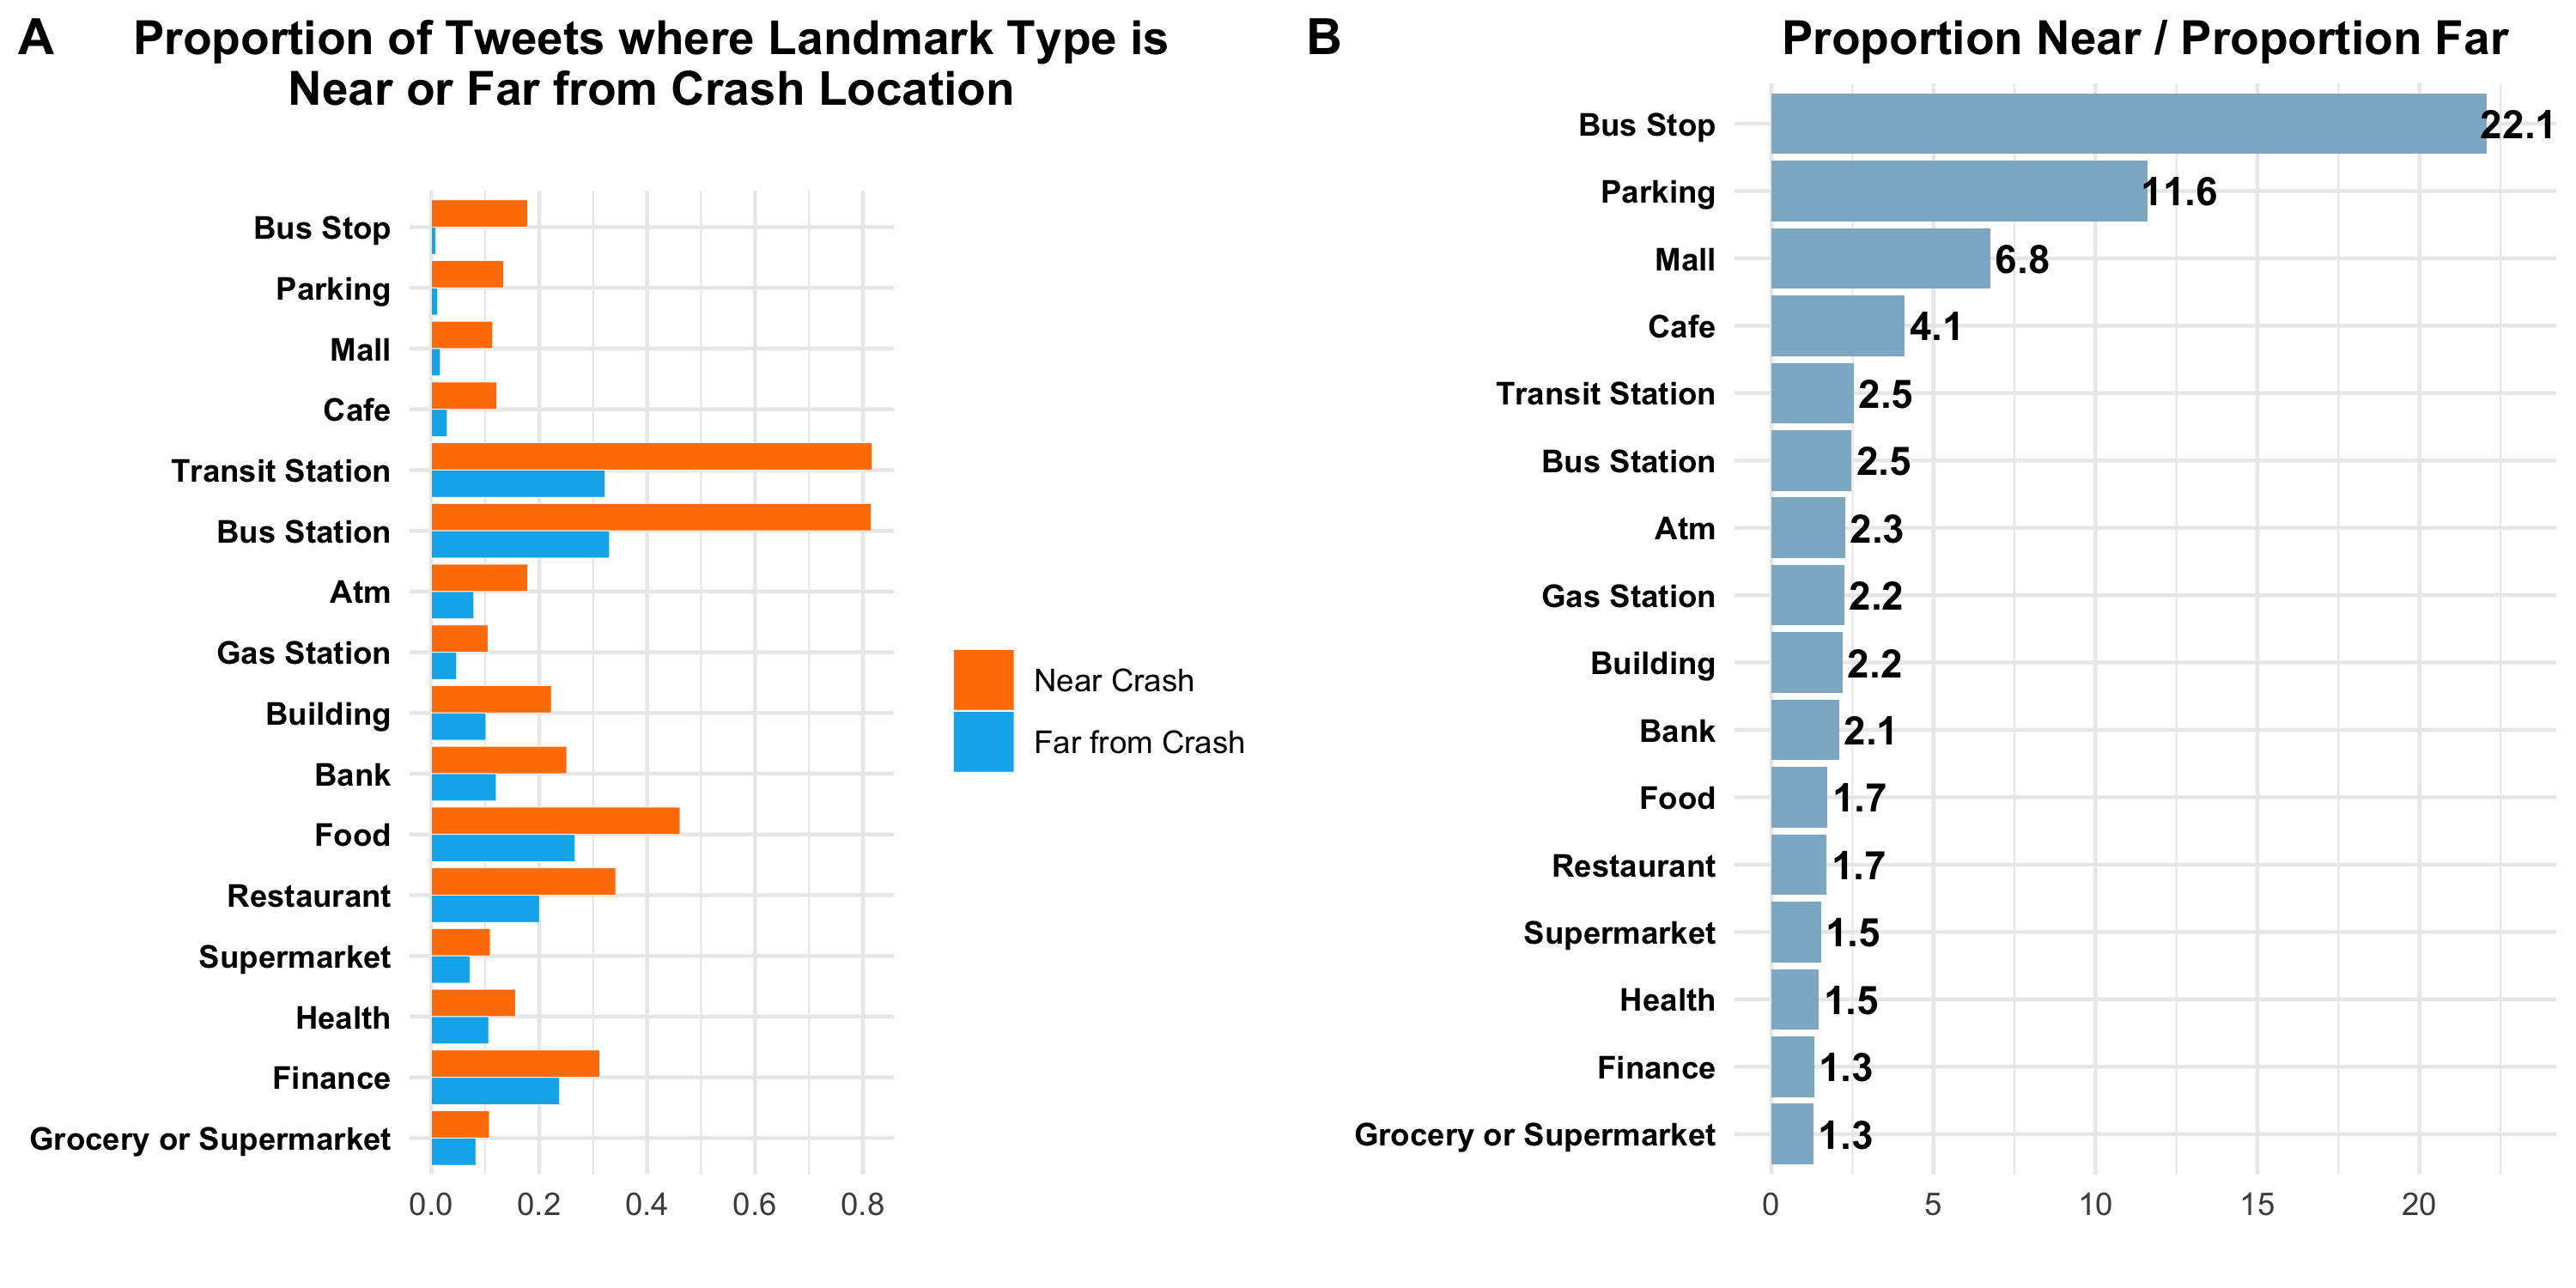
\includegraphics[width=0.75\textwidth]{figures/figure_s2.png}
\caption{In Paper: Figure s2}
\end{figure}

\begin{figure}[H]
\centering
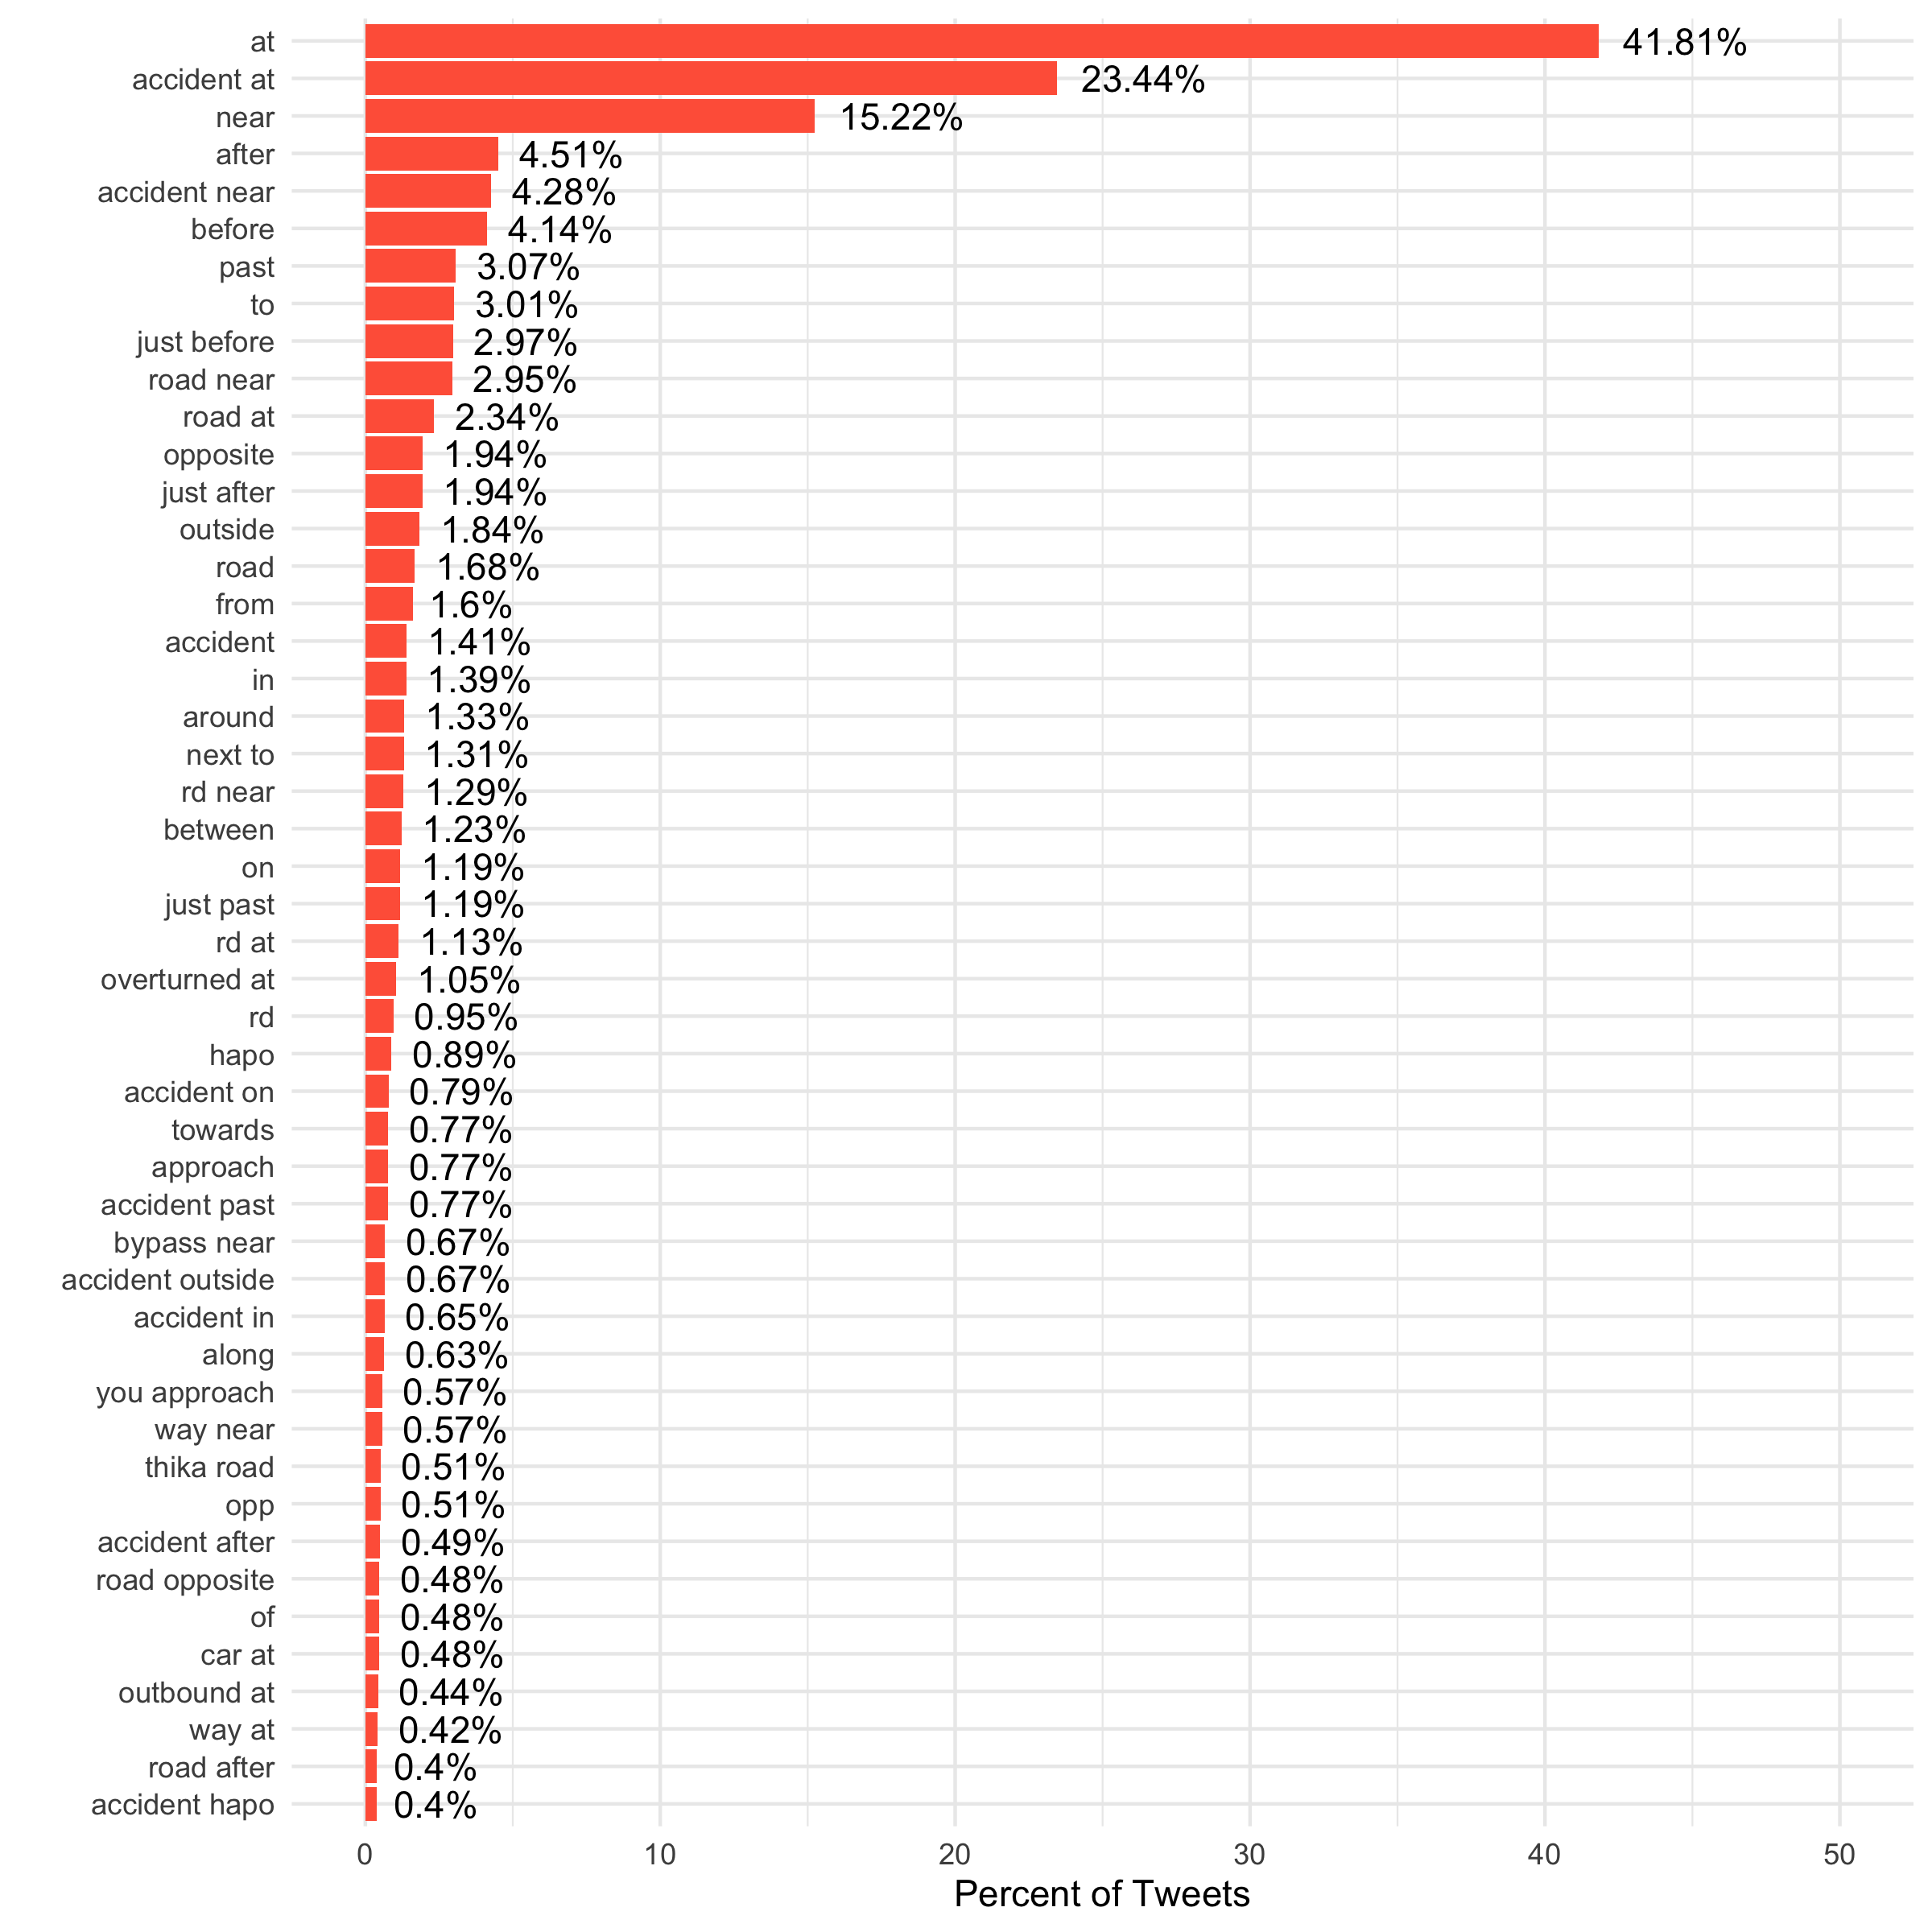
\includegraphics[width=0.75\textwidth]{figures/figure_s3.png}
\caption{In Paper: Figure s3}
\end{figure}

\begin{figure}[H]
\centering
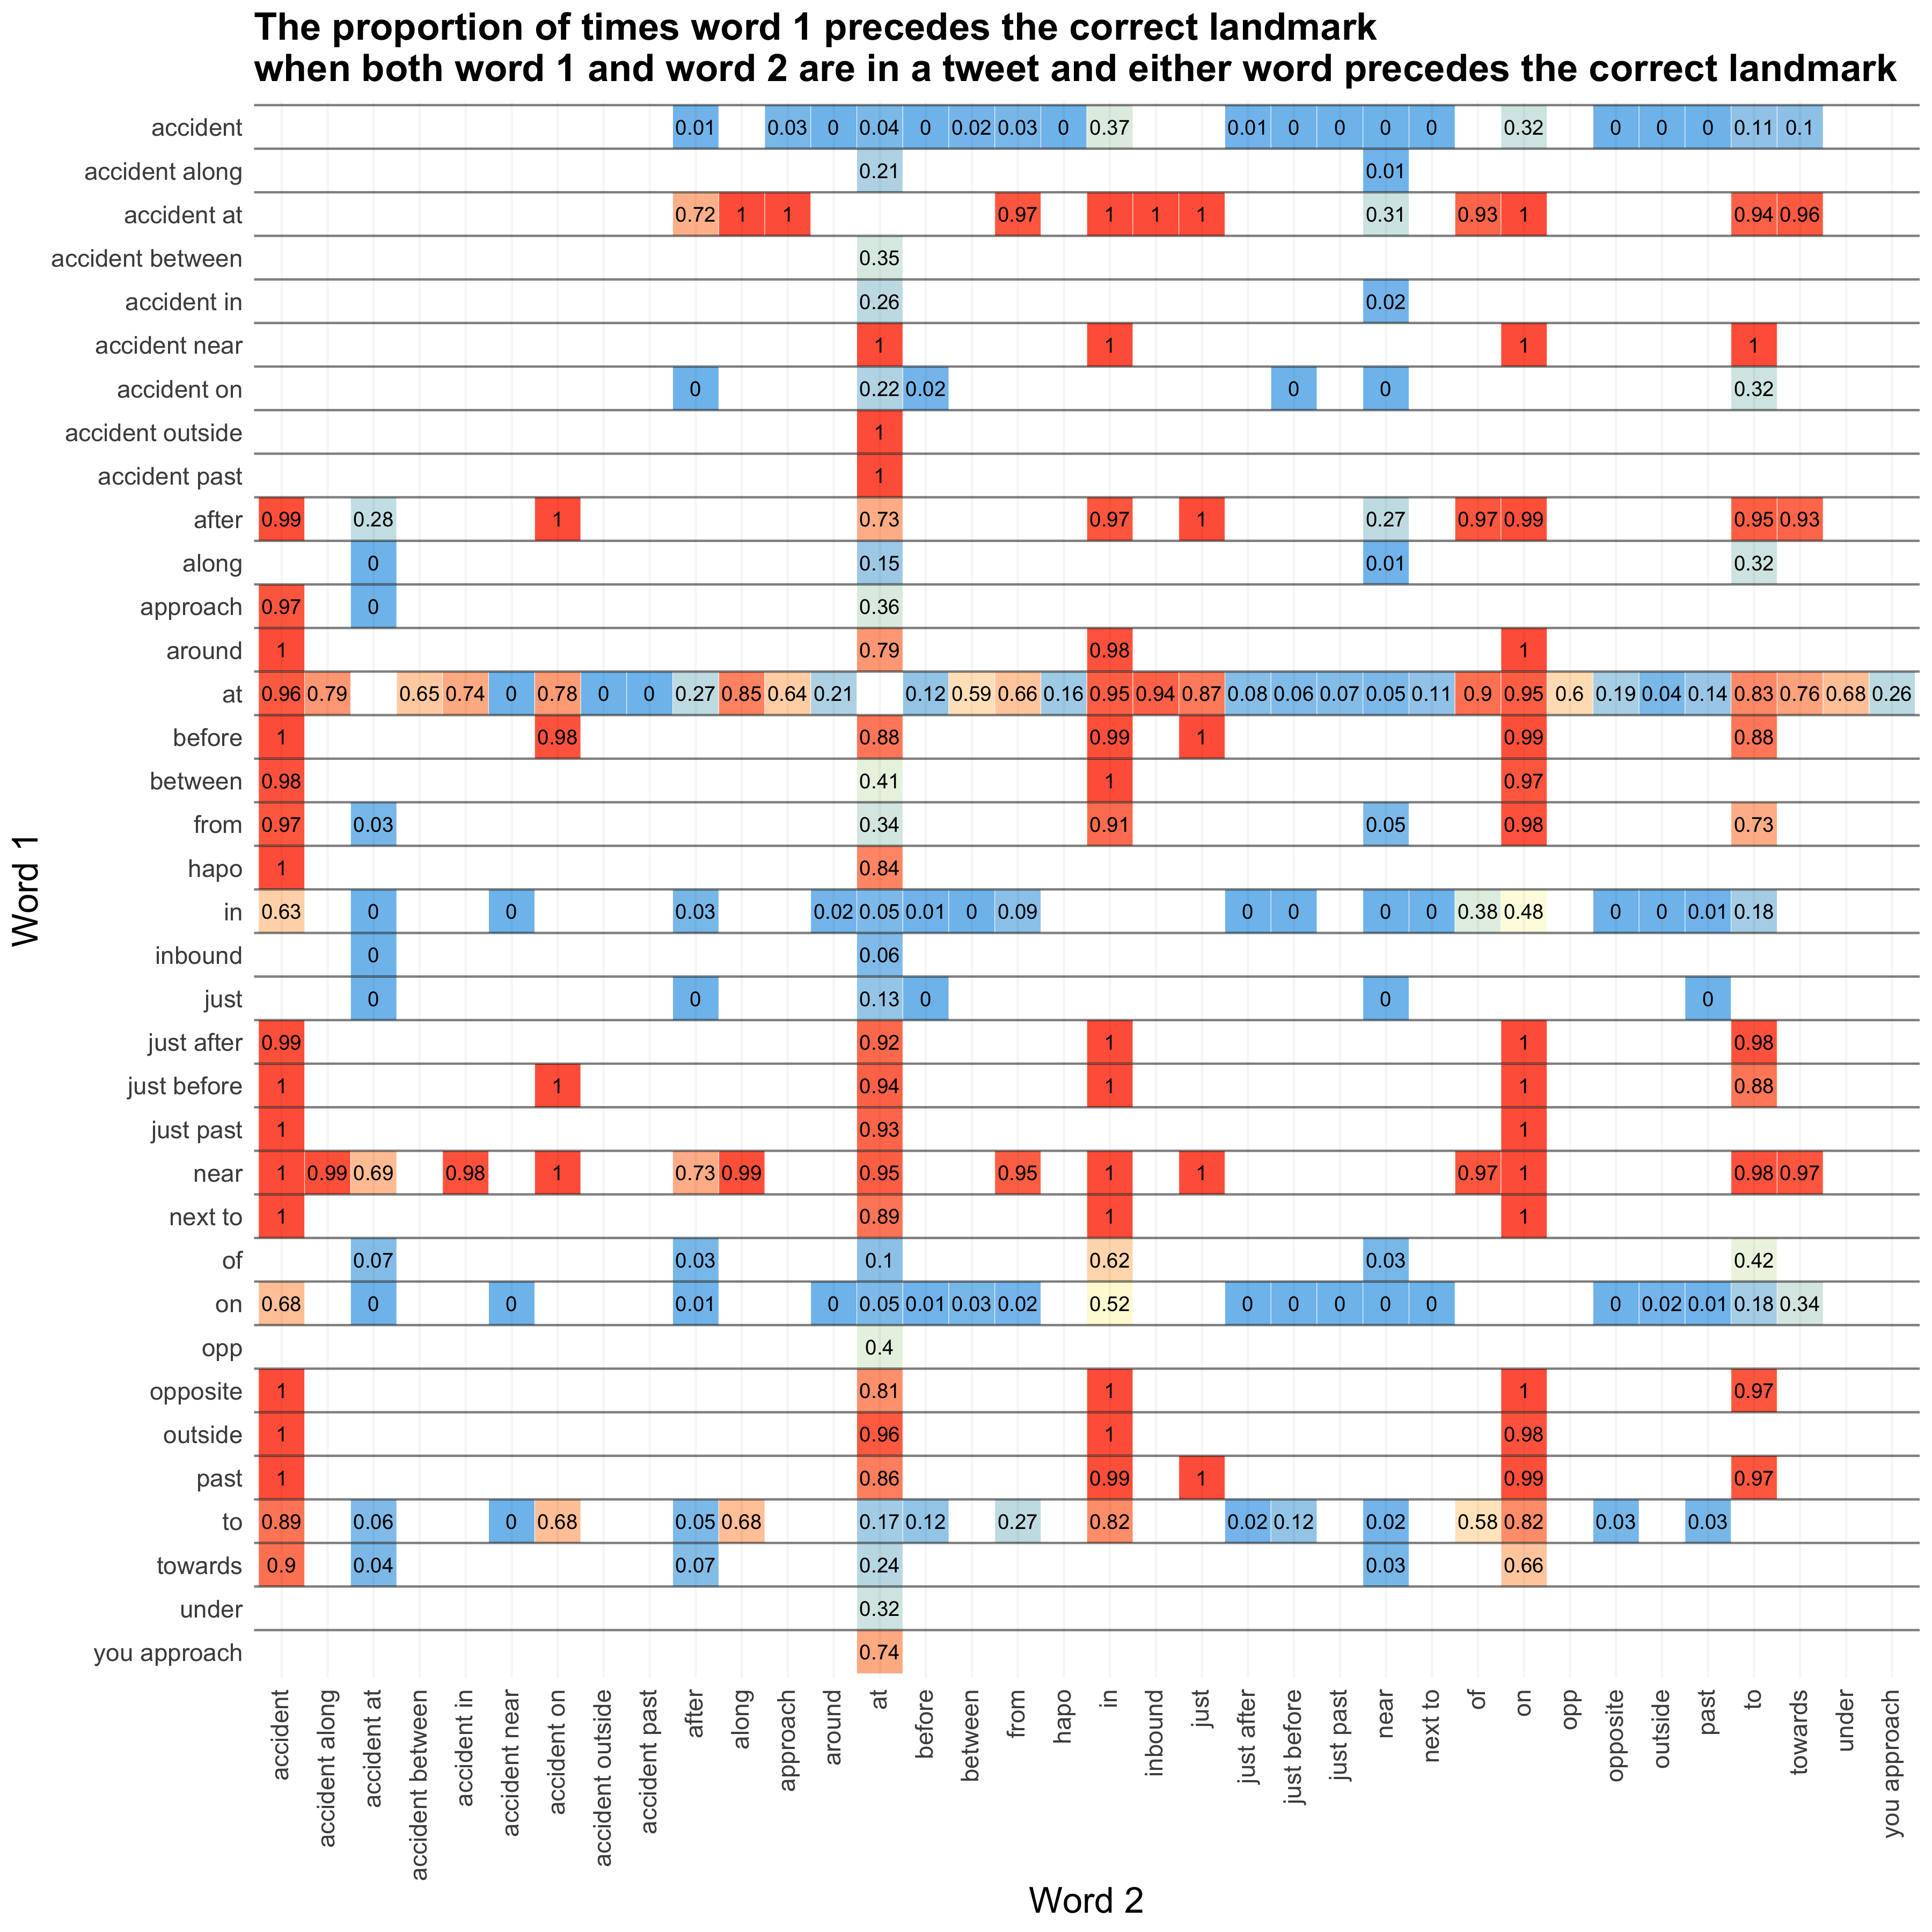
\includegraphics[width=0.75\textwidth]{figures/figure_s4.png}
\caption{In Paper: Figure s4}
\end{figure}

\begin{table}[H]
\caption{In Paper: Table s5}
\centering
\begin{tabular}{l cc | cc | cc } \hline  & \multicolumn{2}{c|}{Any Location Captured by} & \multicolumn{2}{c|}{Crash Location Determined} & \multicolumn{2}{c}{Algorithm Cluster} \\  & \multicolumn{2}{c|}{Algorithm Close to} & \multicolumn{2}{c|}{by Algorithm Close to}  & \multicolumn{2}{c}{Contains} \\  & \multicolumn{2}{c|}{True Crash Location} & \multicolumn{2}{c|}{True Crash Location}  & \multicolumn{2}{c}{True Crash Loction} \\  \hline  & Recall & Precision & Recall & Precision & Recall & Precision \\ \hline \multicolumn{3}{l|}{\bf LNEx} & & & & \\  ~~~ LNEx Aug Gaz & 0.674  &  0.686  &  0.129  &  0.132  &  0.175  &  0.125  \\ \multicolumn{3}{l|}{\bf Algorithm - by Source} & & & & \\  ~~~ Aug Gaz - Geonames & 0.167  &  0.376  &  0.147  &  0.492  &  0.157  &  0.47  \\  ~~~ Aug Gaz - Google & 0.79  &  0.853  &  0.65  &  0.812  &  0.661  &  0.78  \\  ~~~ Aug Gaz - OSM & 0.518  &  0.693  &  0.431  &  0.73  &  0.446  &  0.691  \\ \multicolumn{3}{l|}{\bf Algorithm - All Sources} & & & & \\  ~~~ Raw Gaz & 0.695  &  0.757  &  0.57  &  0.761  &  0.582  &  0.723  \\  ~~~ Aug Gaz & 0.798  &  0.857  &  0.656  &  0.813  &  0.666  &  0.777  \\ \hline \end{tabular} 
\end{table}

\begin{table}[H]
\caption{In Paper: Table s6}
\centering
\begin{tabular}{lcccccc} \hline Variable & Min & Quartile 1 & Median & Mean & Quartile 3 & Max \\ \hline \multicolumn{7}{c}{Truth Dataset 1} \\ Hours Diff  & 0  & 0.133  & 0.508  & 1.473  & 1.482  & 23.776  \\ KMs Diff  & 0  & 0  & 0.004  & 0.202  & 0.112  & 3.407  \\ N Tweets  & 2  & 2  & 2  & 3.283  & 3  & 44  \\ \hline \multicolumn{7}{c}{Truth Dataset 2} \\ Hours Diff  & 0  & 0.157  & 0.547  & 1.529  & 1.746  & 23.417  \\ KMs Diff  & 0  & 0  & 0.018  & 0.253  & 0.179  & 3.407  \\ N Tweets  & 2  & 2  & 2  & 3.274  & 3.5  & 19  \\ \hline \end{tabular} 
\end{table}

\begin{figure}[H]
\centering
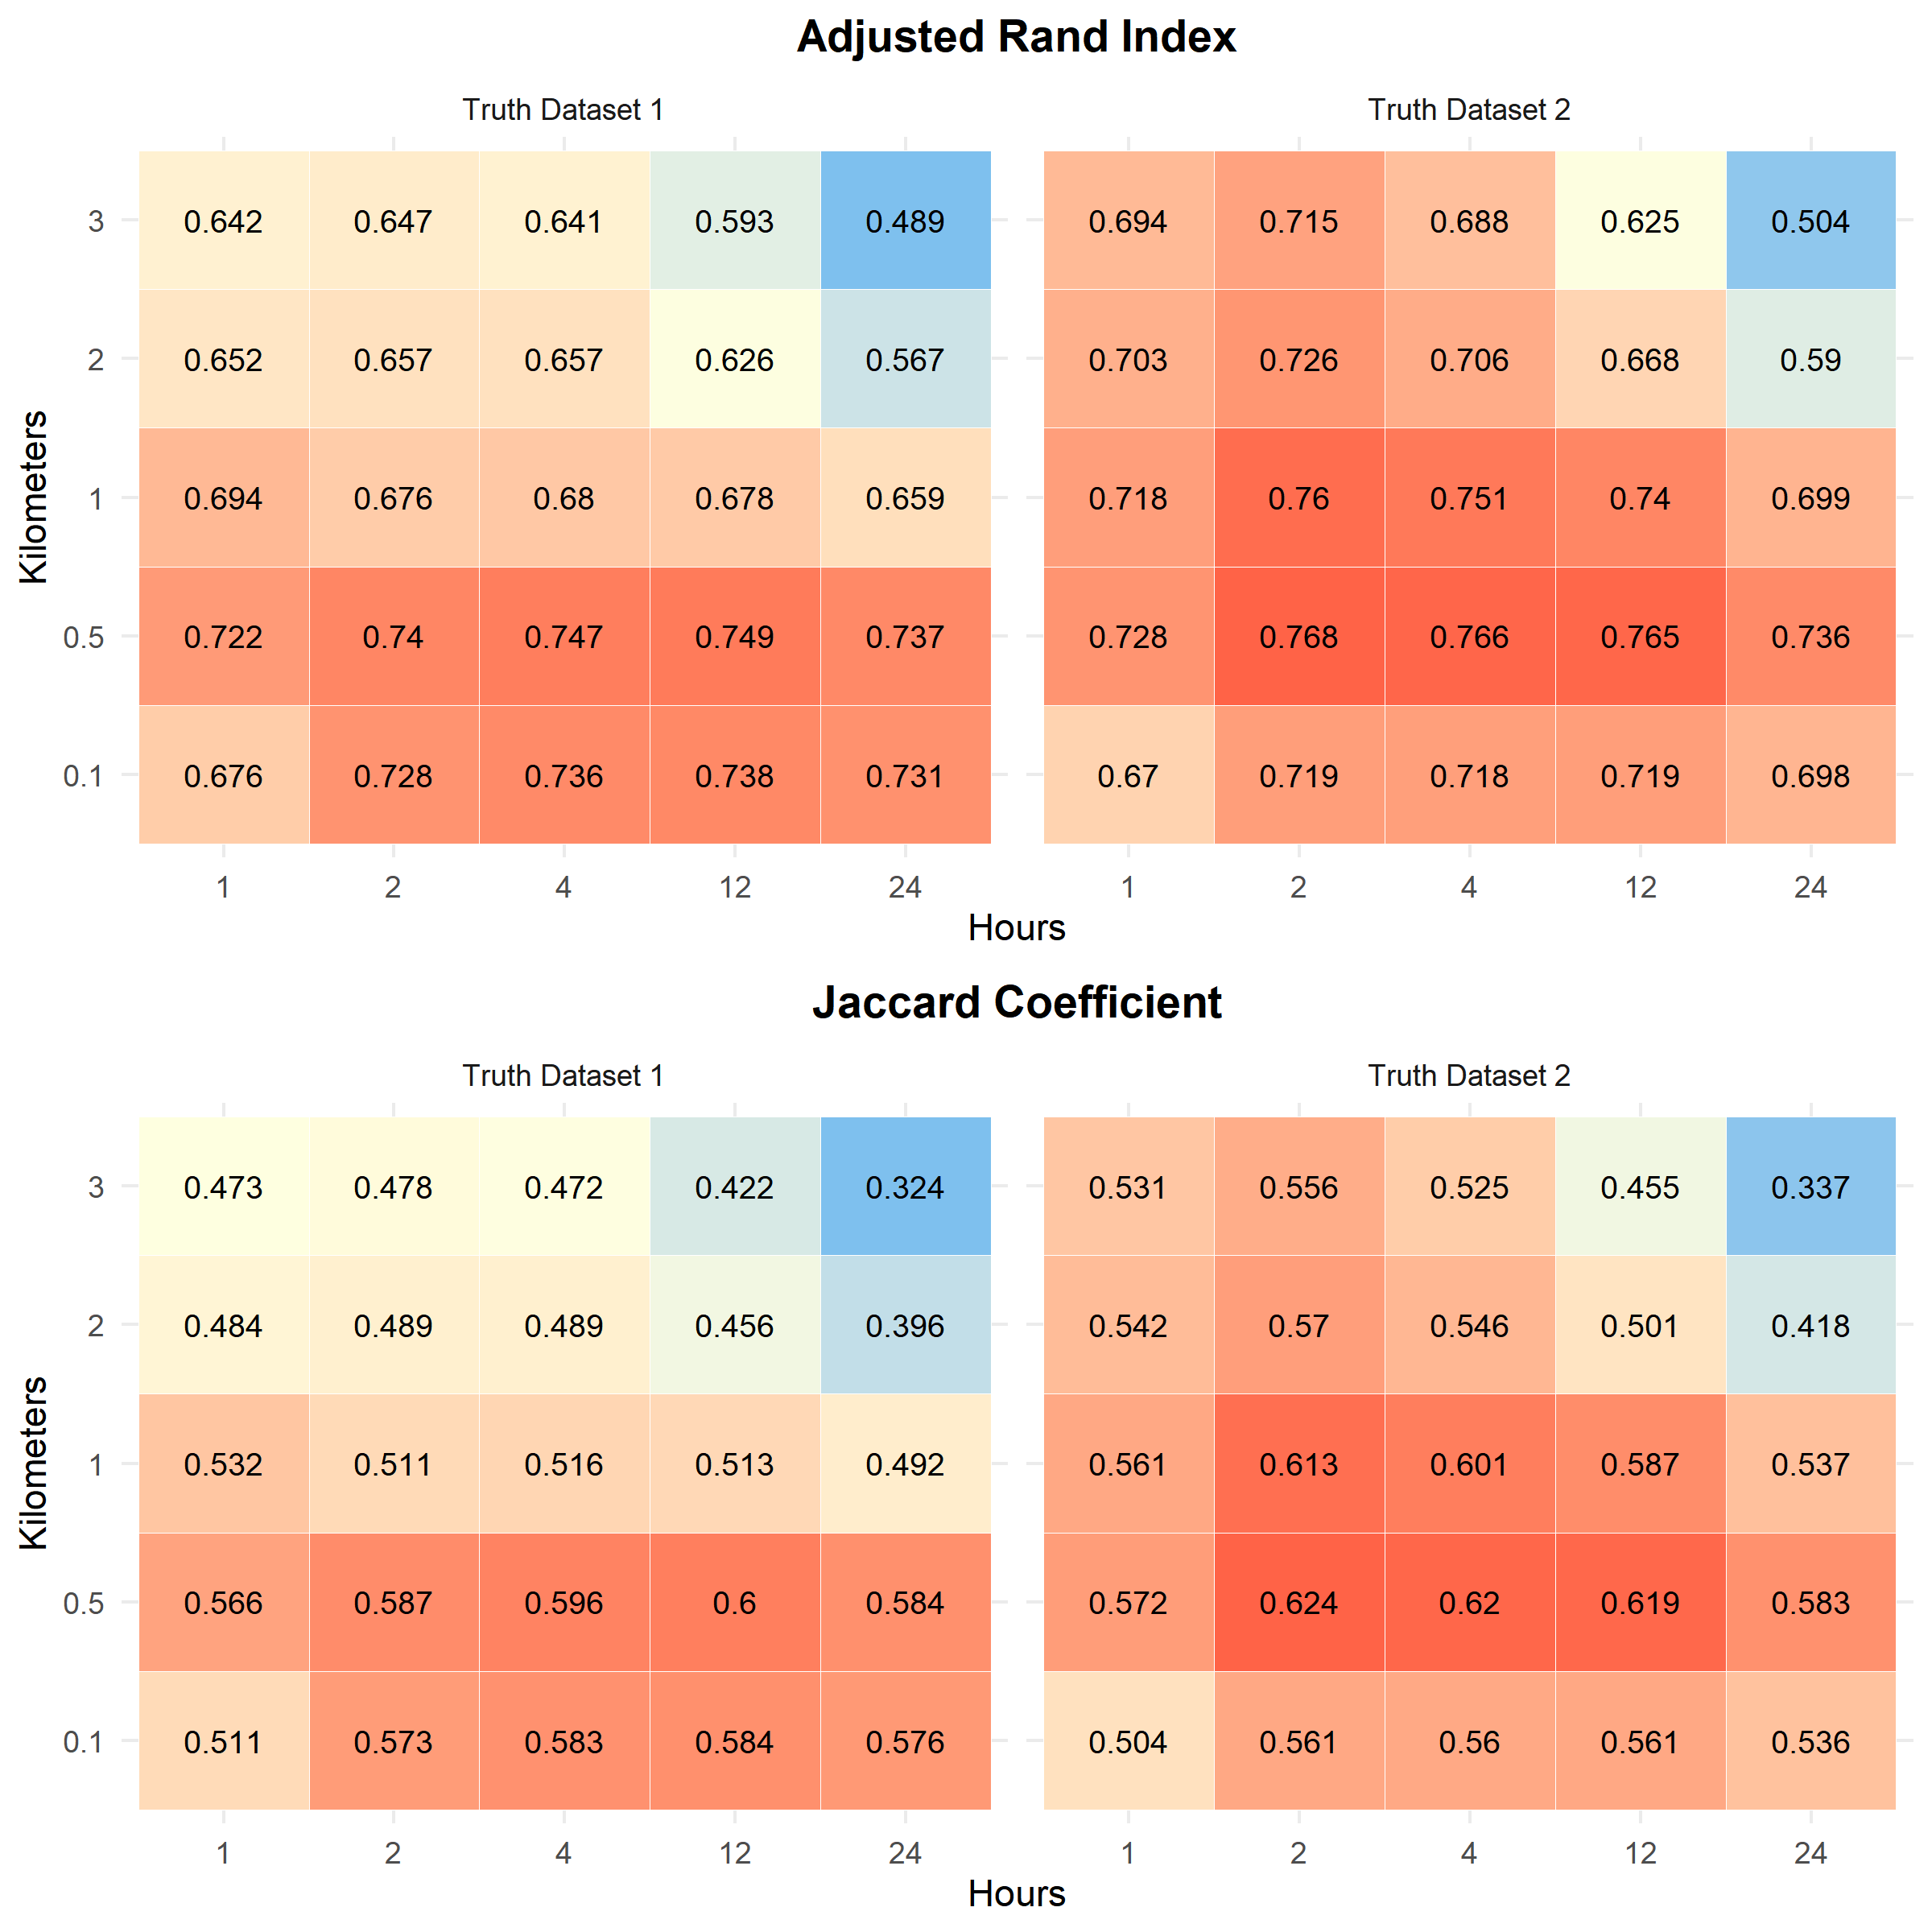
\includegraphics[width=0.75\textwidth]{figures/figure_s5.png}
\caption{In Paper: Figure s5}
\end{figure}


\end{document}  


